\chapter{Fundamentals \textRoman{2}: Linear Optical Response}
\label{cha:fundamentals_b}

% opening paragraph
We continue our discussion of the fundamentals in this chapter, where we introduce the linear optical response of matter.
The interaction between materials and light occurs through the response of electrons to the electric-field component of incident radiation.
This response induces polarization and produces electronic excitations, including interband transitions and plasmonic charge excitations.
Collectively, these processes determine the dielectric function, plasmonic behaviour, absorption, reflection, refraction, and energy loss.
We therefore use linear response theory to connect the electromagnetic field to the dielectric response of the medium.

The discussion follows the route used in the optical analysis of this thesis.
We first introduce the constitutive relations used in the optical calculations, then formulate the dielectric response, and finally derive the optical observables.
The electromagnetic foundations and the detailed causality derivation are given in appendix~\ref{cha:appendix_basic}.
In section~\ref{sec:constitutive_relations_for_optical_response}, we connect the polarization field $\vec{P}(\vec{r},t)$ and electric displacement field $\vec{D}(\vec{r},t)$ to the dielectric tensor $\varepsilon_{\alpha\beta}(\omega)$.
Section~\ref{sec:from_electronic_response_to_dielectric_function} then describes the complex dielectric function $\varepsilon(\omega)=\varepsilon_1(\omega)+i\varepsilon_2(\omega)$ and its directional form in anisotropic media.
Causality constrains the real and imaginary parts of this response, and section~\ref{sec:causality_and_kramers_kronig_relations} expresses this constraint through the Kramers--Kronig relations.
Finally, section~\ref{sec:from_dielectric_function_to_optical_properties} derives the absorption coefficient $\alpha(\omega)$, refractive index $n(\omega)$, extinction coefficient $k(\omega)$, reflectivity $R(\omega)$, and energy-loss spectrum $L(\omega)$ from the complex dielectric function.

\newpage
\section{Constitutive relations for optical response}
\label{sec:constitutive_relations_for_optical_response}

The previous chapter focused on the ground-state electronic problem.
When an electromagnetic field is applied, it drives the electrons away from their static equilibrium and induces polarization.
We therefore start from the relation between the electric field and the induced polarization.
The Maxwell equations, the constitutive relations, and the dielectric tensor are developed in section~\ref{sec:toward_electromagnetic_response_in_matter} of appendix~\ref{cha:appendix_basic}~\cite{landau2013electrodynamics,griffiths2023introduction}.

In this chapter, we use SI units for the macroscopic electrodynamic equations.
The dielectric function is dimensionless and denotes the relative dielectric response.
We use the angular frequency $\omega$ with the time dependence $\exp(-\mathrm{i}\,\omega t)$,
and the photon energy is $\hbar\omega$.

For the linear response in the long-wavelength regime,
we express the polarization field, dielectric tensor, and electric displacement field as:

\begin{equation}
\left\{\begin{aligned}
    P_\alpha(\vec{r},\omega)
    &= \varepsilon_0\sum_\beta\chi_{\alpha\beta}(\omega)E_\beta(\vec{r},\omega) \\
    \varepsilon_{\alpha\beta}(\omega)
    &= \delta_{\alpha\beta}+\chi_{\alpha\beta}(\omega) \\
    D_\alpha(\vec{r},\omega)
    &= \varepsilon_0\sum_\beta\varepsilon_{\alpha\beta}(\omega)E_\beta(\vec{r},\omega)
\end{aligned}\right.
\label{working_constitutive_relations_for_optical_response}
\end{equation}

here, $\chi_{\alpha\beta}(\omega)$ denotes the electric susceptibility tensor,
and $\alpha$ and $\beta$ denote Cartesian components.
These relations connect the applied field to the electric response of the medium.
For the optical response considered here, we neglect magnetic-permeability effects and take $\mu_{\mathrm{r}}(\omega)\approx1$.

When the crystal symmetry allows a diagonal dielectric tensor in the chosen Cartesian axes,
we resolve the response into principal components $\varepsilon_{\lambda\lambda}(\omega)$ with $\lambda=x,y,z$.
We then distinguish the response within the structural plane from the response perpendicular to that plane.
The dielectric tensor therefore provides the starting point for connecting the electronic transitions to the directional optical properties.

\newpage
\section{From electronic response to the dielectric function}
\label{sec:from_electronic_response_to_dielectric_function}

% opening paragraph
The previous section introduced the constitutive relations for optical response.
There, we introduced the polarization field $\vec{P}(\vec{r},t)$,
the electric susceptibility tensor $\chi_{\alpha\beta}(\omega)$,
and the dielectric tensor $\varepsilon_{\alpha\beta}(\omega)$.
These quantities connect the applied field to the response of matter.
We now recover the response function that electronic structure calculations actually provide,
which is the frequency-dependent dielectric function~\cite{onida2002electronic,gajdovs2006linear,ambrosch2006linear}.

In this section, we start by expressing the polarization response in the language of electric susceptibility and the complex dielectric function.
We then identify the microscopic electronic processes that generate its imaginary part.
Next, we formulate this response for anisotropic systems,
since the present work compares the in-plane and out-of-plane optical channels explicitly.
Therefore, we advance from the general constitutive picture to a response function that can be calculated, interpreted, and subsequently converted into optical observables.

\subsection{From polarization response to the complex dielectric function}

Equation~\eqref{working_constitutive_relations_for_optical_response} connects the polarization field $\vec{P}(\vec{r},\omega)$ to the electric susceptibility tensor $\chi_{\alpha\beta}(\omega)$
and the dielectric tensor $\varepsilon_{\alpha\beta}(\omega)$.
We now turn to the dielectric function, which serves as the central quantity in optical response. 
In physical terms, the time-dependent electric field of incident light drives this response by perturbing electrons away from equilibrium and inducing the aforementioned polarization.

The electric susceptibility tensor $\chi_{\alpha\beta}(\omega)$ measures how strongly the polarization component $P_\alpha$ responds to the field component $E_\beta$, while the dielectric tensor $\varepsilon_{\alpha\beta}(\omega)$ collects this response into the form most directly used in optical analysis~\cite{gajdovs2006linear}.

Under a monochromatic electric field, part of the polarization stays in phase with the field,
while another part lags behind it.
The first part stores energy in the medium, and the second part transfers energy from the field into the medium.
We therefore write the dielectric tensor in complex form as:

\begin{equation}
    \varepsilon_{\alpha\beta}(\omega)
    = \varepsilon_{1,\alpha\beta}(\omega)
    + \mathrm{i}\,\varepsilon_{2,\alpha\beta}(\omega)
\label{complex_dielectric_tensor_definition}
\end{equation}

here, $\varepsilon_{1,\alpha\beta}(\omega)$ denotes the real part of the dielectric tensor,
and $\varepsilon_{2,\alpha\beta}(\omega)$ denotes the imaginary part of the dielectric tensor.

The real part denotes the dispersive part of the response.
It describes how the medium polarizes with the field and therefore how it stores electromagnetic energy.

The imaginary part denotes the absorptive part of the response.
It describes how the field drives electronic excitations and therefore how it transfers energy into the medium~\cite{ambrosch2006linear}.

For the later discussion on optical observables,
we consider a decoupled principal-axis mode.
We then suppress the tensor indices and write the dielectric response in scalar form.

Therefore, along a principal direction, the complex dielectric response can be expressed in scalar form as:

\begin{equation}
    \varepsilon(\omega)
    = \varepsilon_1(\omega)
    + \mathrm{i}\,\varepsilon_2(\omega)
\label{complex_dielectric_function_definition}
\end{equation}

here, $\varepsilon_1(\omega)$ denotes the real part of the dielectric function,
and $\varepsilon_2(\omega)$ denotes the imaginary part of the dielectric function.

Under an external electric field, this scalar form represents the dielectric response along a principal direction.
We can therefore derive the absorption coefficient $\alpha(\omega)$,
the refractive index $n(\omega)$,
the extinction coefficient $k(\omega)$,
the reflectivity $R(\omega)$,
and the energy-loss spectrum $L(\omega)$.
This complex dielectric function therefore provides a unified framework for the linear optical properties~\cite{onida2002electronic,djurivsic2002progress,niu2024electronic}.

For the xene systems considered in the present work,
we accordingly resolve the dielectric response for the in-plane and out-of-plane channels for separate analysis.
In anisotropic xenes, the response along the structural plane usually differs substantially from that along the perpendicular direction~\cite{marinopoulos2002anisotropy,huang2023optical,slavich2024exploring,cheng2025two}.

At this stage, we arrive at the complex dielectric function as the central response quantity for discussing optical performance.
When we enter the frequency domain, the optical response no longer appears as a static redistribution of charge;
instead, the field drives the electrons continuously, and the medium responds with a frequency-dependent polarization.
Within this complex quantity, microscopic electronic processes generate the imaginary part $\varepsilon_2(\omega)$,
while the Kramers--Kronig relation determines the real part $\varepsilon_1(\omega)$~\cite{de1926theory, toll1956causality, persson2001first}.
We now turn to the microscopic origin of the imaginary part $\varepsilon_2(\omega)$.

\subsection{Microscopic origin of the imaginary part}

For the complex dielectric function,
the previous subsection discussed that the imaginary part $\varepsilon_2(\omega)$ characterizes the absorptive response of the medium.
We now connect this quantity to the microscopic electronic transitions in the crystal.

When a monochromatic electric field acts on a crystal,
it drives electrons from occupied states to empty states,
and therefore induces interband transitions.
In this process, the external field transfers the energy $\hbar\omega$ to the electronic system,
and the medium absorbs this energy through a dissipative response~\cite{toudert2017interband}.
To describe this dissipative response quantitatively,
we now introduce the optical conductivity tensor $\sigma_{\alpha\beta}(\omega)$ within linear response theory~\cite{kubo1957statistical}.

Firstly, we express the dielectric tensor $\varepsilon_{\alpha\beta}(\omega)$ through the optical conductivity tensor $\sigma_{\alpha\beta}(\omega)$ as~\cite{kubo1957statistical,onida2002electronic}:

\begin{equation}
    \varepsilon_{\alpha\beta}(\omega)
    = \delta_{\alpha\beta} + \frac{\mathrm{i}}{\varepsilon_0\omega}\,
    \sigma_{\alpha\beta}(\omega)
\label{dielectric_tensor_from_optical_conductivity}
\end{equation}

Once we decompose this optical conductivity tensor into its real part $\sigma_{1,\alpha\beta}(\omega)$ and imaginary part $\sigma_{2,\alpha\beta}(\omega)$, 
the previous equation immediately gives:

\begin{equation}
    \varepsilon_{2,\alpha\beta}(\omega)
    = \frac{\sigma_{1,\alpha\beta}(\omega)}{\varepsilon_0\omega}
\label{imaginary_dielectric_from_real_conductivity}
\end{equation}

This relation demonstrates that the imaginary part of the dielectric response directly describes the energy-absorbing part of the induced current,
which leads to dissipation under the external field.

Next, we describe this microscopic process in a periodic solid as a transition from an initial state $\ket{\psi_{n\vec{k}}}$ to a final state $\ket{\psi_{m\vec{k}}}$.
Here, $\vec{k}$ denotes the crystal momentum in the first Brillouin zone.
In the optical regime, the photon momentum is negligible on the scale of the Brillouin zone,
so the transition is effectively vertical in $\vec{k}$-space~\cite{fox2010optical}.
Accordingly, the transition strength is determined by the velocity matrix elements rather than by the band energies alone.

For the present work, we adopt the independent-particle approximation (IPA)
built from the ground-state electronic structure.
We consider the reciprocal electric response and retain the symmetric dielectric tensor,
without its antisymmetric magneto-optical contribution.
The interband part of its imaginary component takes the form~\cite{d2016accurate,gajdovs2006linear}:

\begin{equation}
\begin{aligned}
    \varepsilon_{2,\alpha\beta}^{\mathrm{inter}}(\omega)
    &\propto \frac{1}{\omega^2}\sum_{n\ne m}
    \int_{\mathrm{BZ}}\frac{\dif^3{k}}{(2\pi)^3}\,
    \left(f_{n\vec{k}}-f_{m\vec{k}}\right) \\
    &\quad\times\mathrm{Re}\left[
    \bra{\psi_{m\vec{k}}}\hat{v}_{\alpha}\ket{\psi_{n\vec{k}}}
    \bra{\psi_{n\vec{k}}}\hat{v}_{\beta}\ket{\psi_{m\vec{k}}}
    \right]
    \delta\left(E_{m\vec{k}}-E_{n\vec{k}}-\hbar\omega\right)
\end{aligned}
\label{independent_particle_imaginary_dielectric_tensor}
\end{equation}

here, $n$ and $m$ label the initial and final bands,
and $f_{n\vec{k}}$ and $f_{m\vec{k}}$ denote their occupations.
The band energies $E_{n\vec{k}}$ and $E_{m\vec{k}}$ describe the initial and final states.
The velocity operator $\hat{v}_{\alpha}=(\mathrm{i}/\hbar)[\hat{H},\hat{r}_{\alpha}]$ determines the transition strength along the $\alpha$ direction.
The proportionality sign suppresses a frequency-independent prefactor.
The state labels include spin according to the chosen electronic-structure description.
For a diagonal component, the matrix-element product reduces to
$\left|\bra{\psi_{m\vec{k}}}\hat{v}_{\alpha}\ket{\psi_{n\vec{k}}}\right|^2$.
Meanwhile, the Dirac delta function enforces the energy-conservation condition:

\begin{equation}
    E_{m\vec{k}}-E_{n\vec{k}}=\hbar\omega
\label{dirac_energy_conservation_condition}
\end{equation}

Equation~\eqref{independent_particle_imaginary_dielectric_tensor} describes the microscopic origin of the interband absorptive response.
For a transition to contribute, the occupation difference and the velocity matrix elements must be nonzero,
and the transition energy must match the photon energy $\hbar\omega$.
For an insulator at zero temperature, this reduces to a transition from an occupied valence state to an empty conduction state.
For a metal, the occupations must instead be resolved at each $\vec{k}$.
The corresponding matrix elements therefore serve as the criterion for optically allowed transitions.
When many allowed transitions contribute strongly at the same excitation energy,
a peak can appear in $\varepsilon_{2,\alpha\beta}^{\mathrm{inter}}(\omega)$.

This point clarifies what the calculated spectra describe.
The imaginary part reflects the band energies, the occupation pattern,
and the direction-resolved transition matrix elements.
The Brillouin-zone integration is evaluated using the k-point sampling discussed in section~\ref{subsec:method_kpoints}.
Within the adopted independent-particle description,
the spectra resolve the interband onset, absorption peaks, and directional contrast.
The electron--hole interaction is not included in this approximation.

The tensor indices $\alpha$ and $\beta$ enter directly through the velocity matrix elements.
Therefore, the microscopic transition strength already resolves the field polarization and the crystal directions.
This result naturally leads us to the dielectric response in anisotropic media~\cite{huang2023optical}.

The interband expression does not include the intraband response of free carriers.
For a metal, a simple model for this additional contribution along a principal direction $\lambda$ is the Drude form~\cite{dressel2002electrodynamics}:

\begin{equation}
    \varepsilon_{\lambda\lambda}(\omega)
    = \varepsilon_{\lambda\lambda}^{\mathrm{inter}}(\omega)
    - \frac{\omega_{p,\lambda}^{2}}
    {\omega\left(\omega+\mathrm{i}\,\gamma_{\lambda}\right)}
\label{interband_and_drude_dielectric_response}
\end{equation}

here, $\varepsilon_{\lambda\lambda}^{\mathrm{inter}}(\omega)$ includes the vacuum background of one,
$\omega_{p,\lambda}$ is the plasma angular frequency,
and $\gamma_{\lambda}>0$ is the carrier damping rate.
For the spectra shown here, we use the independent-particle interband response calculated with VASP,
without microscopic local-field effects or a Drude contribution from intraband transitions.
Therefore, these spectra do not describe the complete low-frequency response of the metallic systems.

\subsection{Dielectric response in anisotropic media}

The previous subsection established the microscopic expression for the interband part of the imaginary dielectric response.
We now describe the dielectric response of anisotropic media in a direction-resolved form~\cite{slavich2024exploring}.

For an anisotropic medium, once we determine the principal directions,
equation~\eqref{principal_axis_dielectric_tensor} describes the principal-axis form of the dielectric tensor $\varepsilon_{\alpha\beta}(\omega)$.
For each principal component with $\lambda=x,y,z$, 
we write the complex dielectric function in a direction-resolved form~\cite{nye1985physical}:

\begin{equation}
    \varepsilon_{\lambda\lambda}(\omega) =
    \varepsilon_{1,\lambda\lambda}(\omega)
    + \mathrm{i}\,\varepsilon_{2,\lambda\lambda}(\omega)
\label{direction_resolved_complex_dielectric_function}
\end{equation}

here, the real part $\varepsilon_{1,\lambda\lambda}(\omega)$ describes the directional dispersive response,
whereas the imaginary part $\varepsilon_{2,\lambda\lambda}(\omega)$ describes the directional absorptive response.
As different principal components produce different optical responses along different directions, 
optical anisotropy appears~\cite{nye1985physical}.

In what follows,
we denote the dielectric response within the structural plane by the in-plane dielectric function $\varepsilon_{\varparallel}(\omega)$,
whereas we denote the response normal to that plane by
the out-of-plane dielectric function $\varepsilon_{\perp}(\omega)$.

Once we decompose the dielectric response into directional channels,
the derived optical properties inherit the same anisotropy~\cite{alonso2004optical}.

A representative example of the direction-resolved dielectric response is shown in the following figure.
The real and imaginary parts exhibit distinct in-plane and out-of-plane features over the full photon-energy range.
The $\alpha$-Beryllene and $\beta$-Beryllene spectra in this chapter were calculated by the author for the study presented in chapter~\ref{cha:project_beryllene}.
The calculation methods and corresponding optical results are discussed in sections~\ref{3_methods} and~\ref{3_optical_alpha_beta}.

For these two-dimensional systems, the calculated dielectric response includes the vacuum region of the supercell.
We use the optical volume normalization adopted in chapter~\ref{cha:project_beryllene}~\cite{yang2021method}:

\begin{equation}
\left\{\begin{aligned}
    \varepsilon_{1,\lambda\lambda}^{\mathrm{2D}}(\omega)
    &= 1+\frac{d_{\mathrm{SC}}}{d_{\mathrm{2D}}}
    \left[\varepsilon_{1,\lambda\lambda}^{\mathrm{SC}}(\omega)-1\right] \\
    \varepsilon_{2,\lambda\lambda}^{\mathrm{2D}}(\omega)
    &= \frac{d_{\mathrm{SC}}}{d_{\mathrm{2D}}}
    \varepsilon_{2,\lambda\lambda}^{\mathrm{SC}}(\omega)
\end{aligned}\right.
\label{optical_volume_normalization_2d}
\end{equation}

here, $d_{\mathrm{SC}}$ is the full supercell height,
and $d_{\mathrm{2D}}$ is the chosen effective thickness of the layer.
The superscripts $\mathrm{SC}$ and $\mathrm{2D}$ distinguish the supercell response from the normalized response.
The thickness values are given in section~\ref{3_supplementary}.
The dielectric function and the derived optical quantities therefore remain associated with this thickness convention.

\begin{figure}[htbp]
\centering
    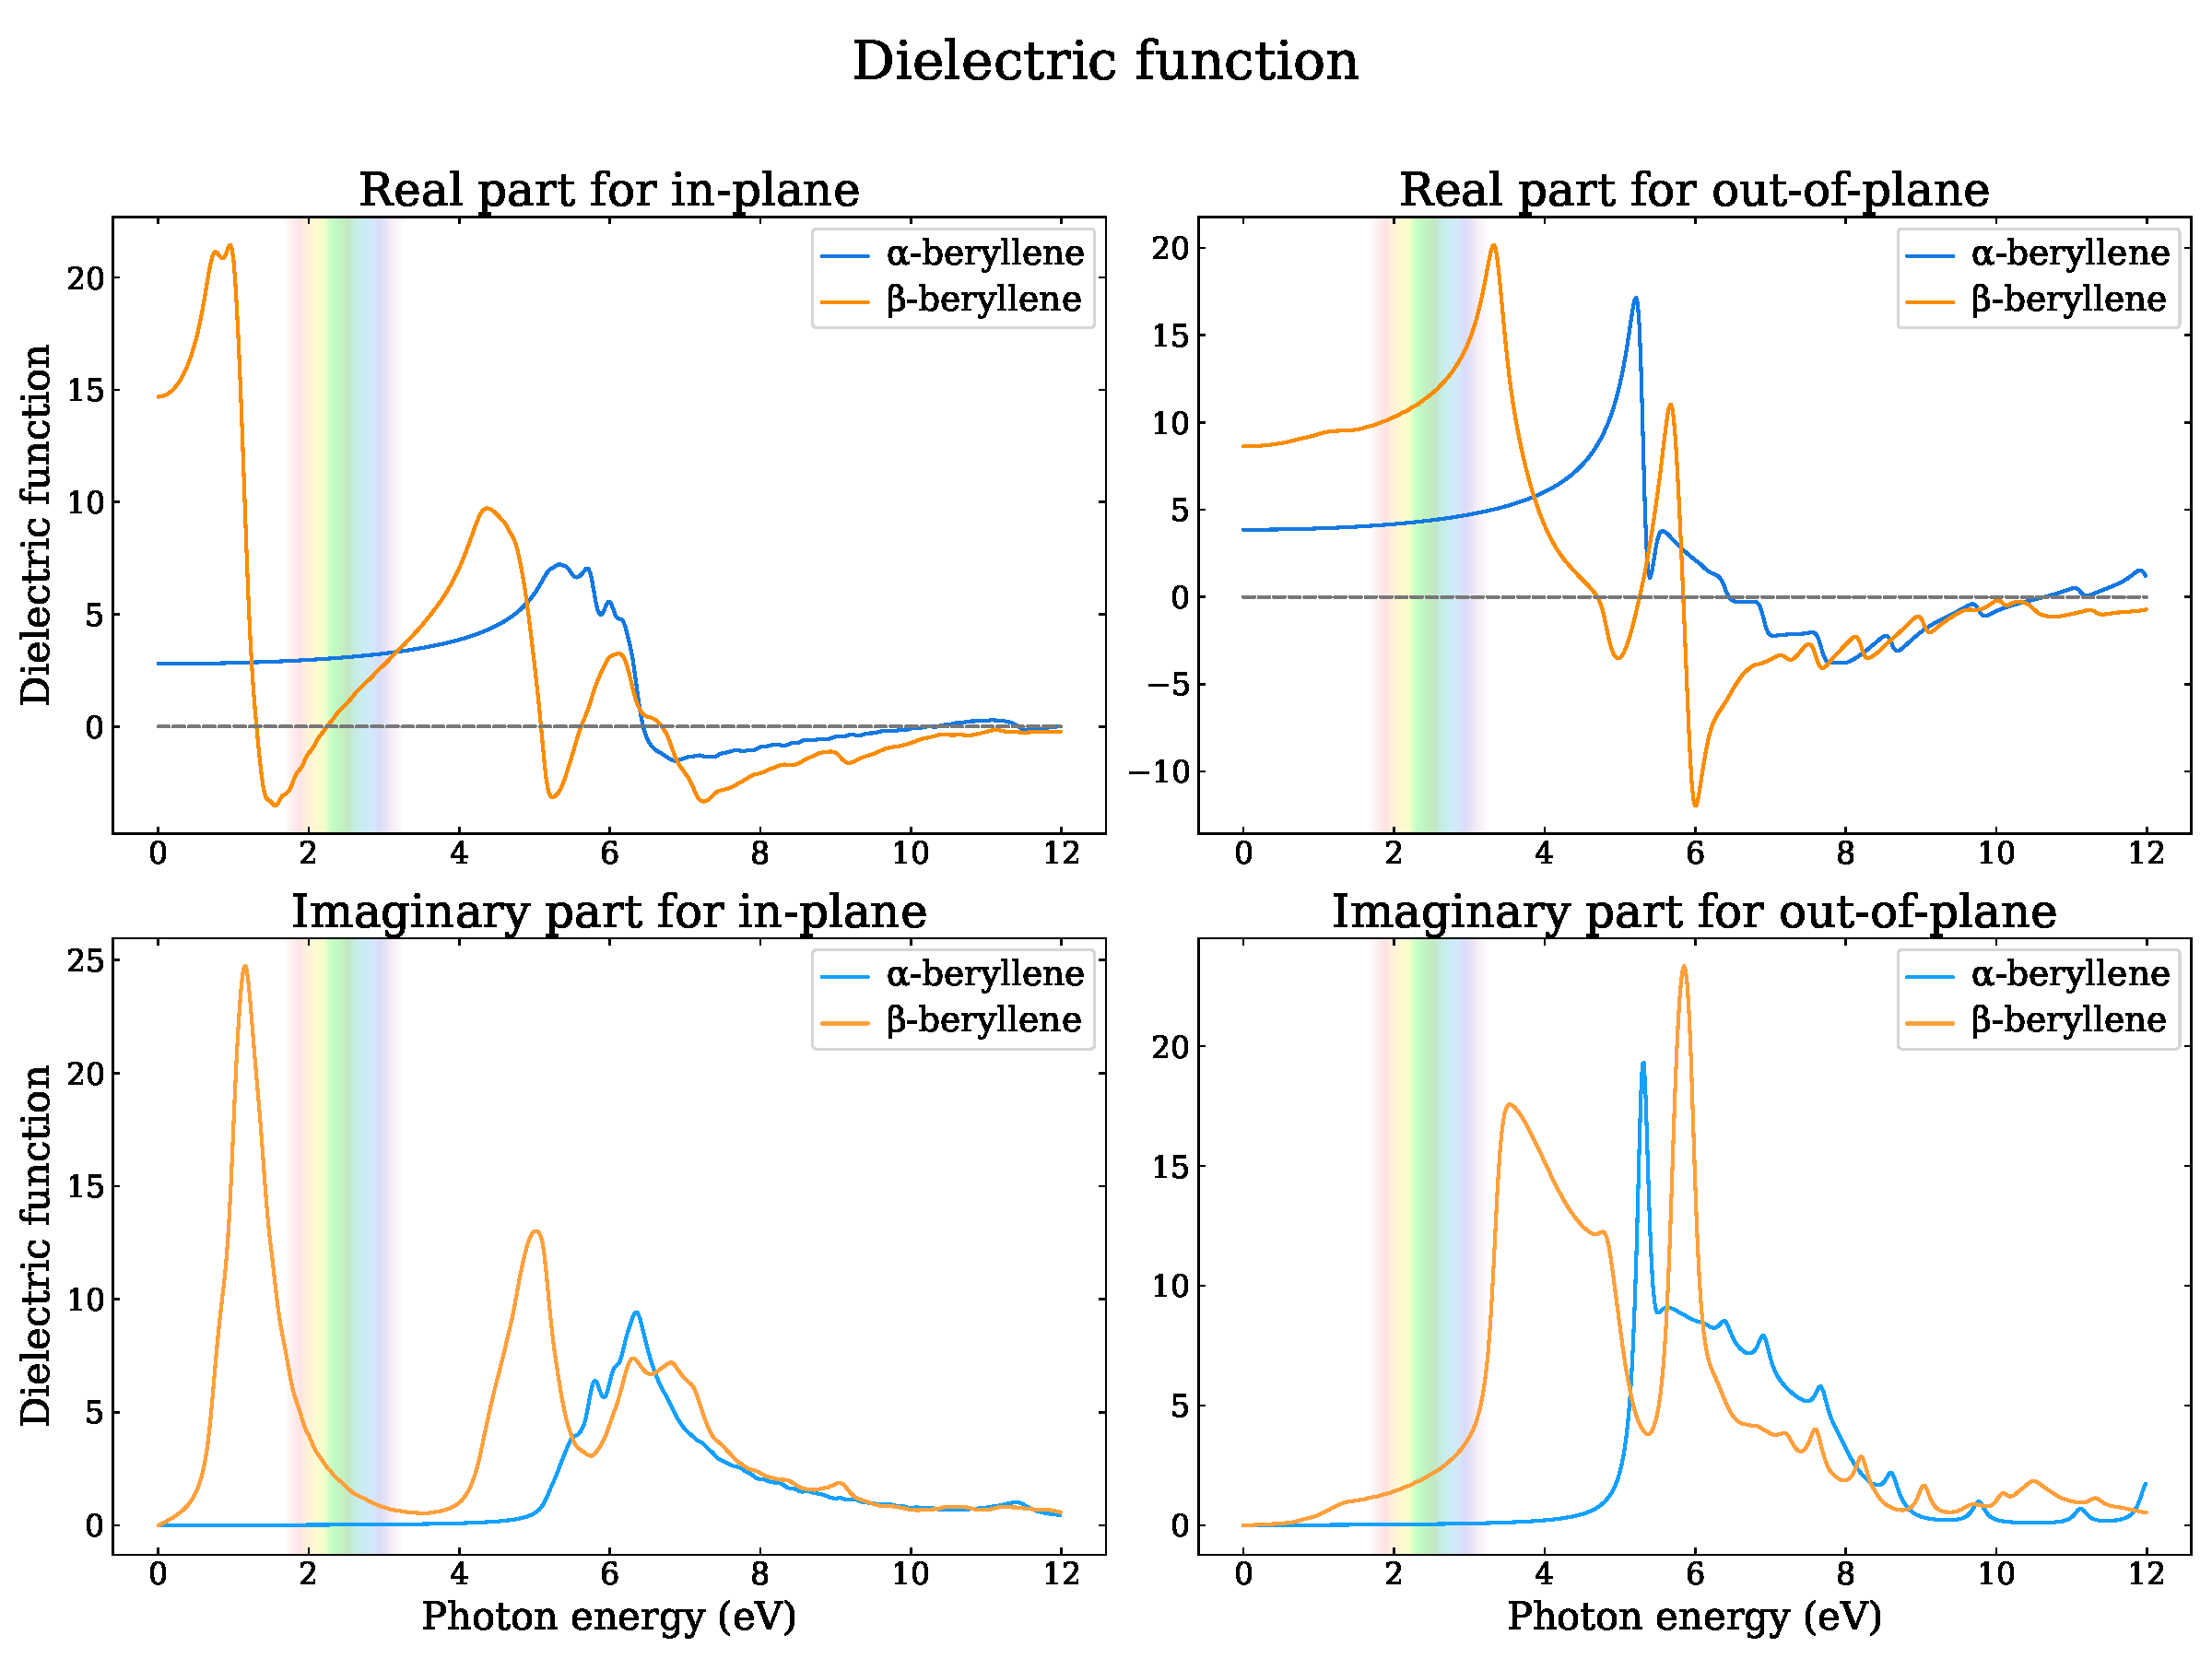
\includegraphics[width=0.95\textwidth]{figures_ch3/3.1_dielectric.pdf}
\caption{Representative real and imaginary parts of the in-plane and out-of-plane dielectric function as a function of photon energy for $\alpha$-Beryllene and $\beta$-Beryllene. The figure illustrates the direction-resolved complex dielectric response discussed in the text.
The in-plane and out-of-plane curves correspond to the $xx$ and $zz$ components, respectively.
These spectra are from our calculations presented in chapter~\ref{cha:project_beryllene}.}
\label{figure_representative_dielectric_response}
\end{figure}

At this stage, we have established the direction-resolved complex dielectric response for anisotropic media.
For each principal direction, the real and imaginary parts are not independent.
In the next section,
we introduce causality as the fundamental constraint on the linear response,
and then derive the Kramers--Kronig relations for each directional component.

\newpage
\section{Causality and the Kramers--Kronig relations}
\label{sec:causality_and_kramers_kronig_relations}

% opening paragraph
The previous section established a direction-resolved complex dielectric response for anisotropic media.
We now identify the constraint that connects the real and imaginary parts of each directional component.

Here, the major physical constraint is causality~\cite{toll1956causality}.
Specifically, causality means that the polarization response cannot occur before the external electric field is applied.
Equivalently, in the time domain, the response kernel vanishes when the response time precedes the driving time.
This temporal order determines the analytic structure of the response function in frequency space.
As a result, for each complex component,
the real and imaginary parts cannot vary independently;
instead, they are related through the Kramers--Kronig relations~\cite{de1926theory, toll1956causality, lucarini2005kramers}.

Therefore, for the dielectric response, once we calculate the absorptive part,
we can determine the dispersive part and construct the complete dielectric response.
This connection completes the dielectric response and opens the derivation of the optical properties.

\subsection{Kramers--Kronig relations for the dielectric function}

The analytic structure of the dielectric response is derived in section~\ref{sec:causality_derivation_basic} of appendix~\ref{cha:appendix_basic}.
We now use this causal structure to connect the real and imaginary parts of the dielectric function~\cite{toll1956causality}.
Here, we consider the regular electronic response without a zero-frequency conductivity pole,
with $\varepsilon_{\alpha\beta}(\omega)\to\delta_{\alpha\beta}$ at high frequency.
For a metal, the conductive term must be separated before applying these relations in the form below.
The dielectric function in this derivation then denotes the remaining regular response.

The symmetry relations in equation~\eqref{parity_of_dielectric_components} reduce the full-frequency integrals to positive-frequency integrals.
In the principal-axis representation,
each complex dielectric component $\varepsilon_{\lambda\lambda}(\omega)$ satisfies the Kramers--Kronig relations in the form~\cite{ossikovski2021constitutive}:

\begin{equation}
\left\{\begin{aligned}
    \varepsilon_{1,\lambda\lambda}(\omega) &=
    1+\frac{2}{\pi}\mathcal{P}
    \int_{0}^{\infty}\dif{\omega'}\,
    \frac{\omega'\varepsilon_{2,\lambda\lambda}(\omega')}{\omega'^2-\omega^2} \\
    \varepsilon_{2,\lambda\lambda}(\omega) &=
    -\frac{2\omega}{\pi}\mathcal{P}
    \int_{0}^{\infty}\dif{\omega'}\,
    \frac{\varepsilon_{1,\lambda\lambda}(\omega')-1}{\omega'^2-\omega^2}  
\end{aligned}\right.
\label{kk_positive_frequency_dielectric_component}
\end{equation}

here, $\mathcal{P}$ denotes the Cauchy principal value.

These relations provide the positive-frequency form of the dielectric response in the present work.
Once we obtain the absorptive part $\varepsilon_{2,\lambda\lambda}(\omega)$ from the electronic transitions,
equation~\eqref{kk_positive_frequency_dielectric_component} determines the dispersive part $\varepsilon_{1,\lambda\lambda}(\omega)$.
This relation also preserves the causal connection between the two parts of the dielectric response.

Consequently, the complex dielectric function describes the absorptive
and dispersive responses of the medium within a unified framework.
The imaginary part characterizes the energy absorbed by the medium at a given frequency,
whereas the real part describes the associated dispersion generated by the same response process.
Within this framework, equation~\eqref{kk_positive_frequency_dielectric_component} directly determines the static limit.
In the next subsection, we derive the corresponding static expression and clarify its physical meaning.

\subsection{Static limit and physical interpretation}

The previous subsection established the positive-frequency form of the Kramers--Kronig relations for the dielectric response.
We now describe the static limit and clarify its physical interpretation~\cite{onishi2024universal,vandenberghe2023two}.

Firstly, for the regular electronic response with a convergent static integral,
we set $\omega\to0$ in the positive-frequency Kramers--Kronig relations~\eqref{kk_positive_frequency_dielectric_component}.
This limit does not represent the full static dielectric response of a conducting system.
We then obtain the static electronic response in the principal-axis representation:

\begin{equation}
    \varepsilon_{1,\lambda\lambda}(0)
    = 1+\frac{2}{\pi}
    \int_{0}^{\infty}\dif{\omega'}\,
    \frac{\varepsilon_{2,\lambda\lambda}(\omega')}{\omega'}
\label{static_limit_from_kramers_kronig}
\end{equation}

here, $\varepsilon_{1,\lambda\lambda}(0)$ characterizes the static dielectric response along the principal direction $\lambda$.
This expression shows that the static limit is not an independent quantity;
instead, the full directional absorption spectrum $\varepsilon_{2,\lambda\lambda}(\omega)$ determines it through causality~\cite{osanloo2021identification}.

Next, the factor $1/\omega'$ gives higher weight to low-energy spectral contributions.
The dominant contribution nevertheless depends on the spectral weight over the full energy range.
Therefore, the static limit represents an accumulated response over the full absorption spectrum.

Meanwhile, anisotropic media generally exhibit different spectral-weight distributions along different principal directions~\cite{suk2024ultrafast,sun2025recent}.

The Kramers--Kronig relations~\eqref{static_limit_from_kramers_kronig} describe a direct directional dependence in the static limit.
The different directional absorption spectra produce different directional static dielectric responses~\cite{suk2024ultrafast}.

Consequently, the static limit reveals the physical interpretation of the Kramers--Kronig relations.
The imaginary part characterizes the spectral weight generated by electronic excitations, 
whereas the real part determines the corresponding zero-frequency dielectric response.
Therefore, the complex dielectric function provides the complete information required for the subsequent optical properties~\cite{lucarini2005kramers,vandenberghe2023two}.

We next use the same dielectric response to derive the absorption coefficient, refractive index, extinction coefficient, reflectivity, and energy-loss spectrum.

\newpage
\section{From the dielectric function to optical properties}
\label{sec:from_dielectric_function_to_optical_properties}

% opening paragraph
The previous section established the complex dielectric function.
It describes the optical response of the present systems.
We now apply this dielectric response to determine the
corresponding optical properties.

We start from the absorption coefficient $\alpha(\omega)$,
which characterizes the attenuation of incident light in the
medium.
We then turn to the refractive index $n(\omega)$ and extinction
coefficient $k(\omega)$, which describe phase propagation and
amplitude decay.
Next, we determine the reflectivity $R(\omega)$, which
represents the reflected portion of the electromagnetic wave at
the interface.
Finally, we examine the energy-loss spectrum $L(\omega)$,
which identifies the dominant resonant energy-loss channels in the medium.

In what follows, we present the general relations that
connect these quantities to the complex dielectric function $\varepsilon(\omega)$~\cite{born2013principles,wooten2013optical,dressel2002electrodynamics,fox2010optical}.
Recent first-principles studies have also analyzed the dielectric response together with the derived optical properties in low-dimensional materials~\cite{niu2024electronic,khan2025insight,albert2024optical,huang2023optical,cheng2025two}.
Afterwards, we analyze the in-plane and out-of-plane optical response of the present systems.
For absorption, refraction, and reflection, we use the local effective-medium description of a transverse principal-axis mode with $\mu_{\mathrm{r}}(\omega)\approx1$.
The index $\lambda$ denotes the electric-field polarization.
In the propagation equations, $z$ denotes distance along the wave path and need not coincide with the structural out-of-plane axis.

\subsection{Absorption coefficient}

We first consider the absorption coefficient $\alpha_{\lambda}(\omega)$,
which characterizes the optical attenuation for polarization along the principal direction $\lambda$~\cite{lin2023recent}.

For a monochromatic wave propagating through the medium,
the intensity follows:

\begin{equation}
    I_{\lambda}(z,\omega)= I_{\lambda,0}(\omega)\,e^{-\alpha_{\lambda}(\omega) z}
\label{intensity_attenuation_from_absorption_coefficient}
\end{equation}

here, we use $z$ to represent the propagation distance in the medium.
$I_{\lambda,0}(\omega)$ is the intensity just inside the medium at $z=0$,
and $I_{\lambda}(z,\omega)$ is the intensity at depth $z$.
Therefore, a larger absorption coefficient corresponds to
stronger attenuation and shorter optical penetration depth.

We next introduce the complex refractive index along the
principal direction $\lambda$:

\begin{equation}
    N_{\lambda}(\omega) = n_{\lambda}(\omega) +\mathrm{i}\, k_{\lambda}(\omega)
\label{complex_refractive_index_for_absorption_coefficient}
\end{equation}

here, $n_{\lambda}(\omega)$ denotes the refractive index,
whereas $k_{\lambda}(\omega)$ denotes the extinction coefficient.
We then express the absorption coefficient $\alpha_{\lambda}(\omega)$ as:

\begin{equation}
    \alpha_{\lambda}(\omega)
    = \frac{2\,\omega}{c}k_{\lambda}(\omega)
\label{absorption_coefficient_from_extinction_coefficient}
\end{equation}

here, $c$ is the speed of light in vacuum.
This expression connects the absorption coefficient to the imaginary part of the complex refractive index.
That imaginary part drives the amplitude decay in the medium~\cite{wooten2013optical, dressel2002electrodynamics,fox2010optical,gajdovs2006linear}.

We now combine the defining relation between the complex
refractive index $N_{\lambda}(\omega)$
and the complex dielectric function $\varepsilon_{\lambda\lambda}(\omega)$ as~\cite{born2013principles}:

\begin{equation}
    N_{\lambda}^{2}(\omega)= \varepsilon_{\lambda\lambda}(\omega)
\label{refractive_index_dielectric_relation}
\end{equation}

Using this relation together with equation~\eqref{direction_resolved_complex_dielectric_function},
we then derive the absorption coefficient $\alpha_{\lambda}(\omega)$ from the complex dielectric function $\varepsilon_{\lambda\lambda}(\omega)$~\cite{born2013principles}:

\begin{equation}
    \alpha_{\lambda}(\omega)
    = \frac{\sqrt{2}\,\omega}{c}
    \left[\sqrt{\varepsilon_{1,\lambda\lambda}^{2}(\omega)
        + \varepsilon_{2,\lambda\lambda}^{2}(\omega)}
        - \varepsilon_{1,\lambda\lambda}(\omega)\right]^{1/2}
\label{absorption_coefficient_from_dielectric_function}
\end{equation}

This equation expresses the absorption coefficient as a
response quantity derived from the dielectric function.
Here, the imaginary part $\varepsilon_{2,\lambda\lambda}(\omega)$ provides the spectral weight generated by electronic transitions,
whereas the real part $\varepsilon_{1,\lambda\lambda}(\omega)$ modifies the magnitude and energy dependence of the resulting attenuation.

The following figure presents the calculated absorption coefficient $\alpha_{\lambda}(\omega)$ spectra of the present systems for the in-plane and out-of-plane directions:

\begin{figure}[htbp]
\centering
    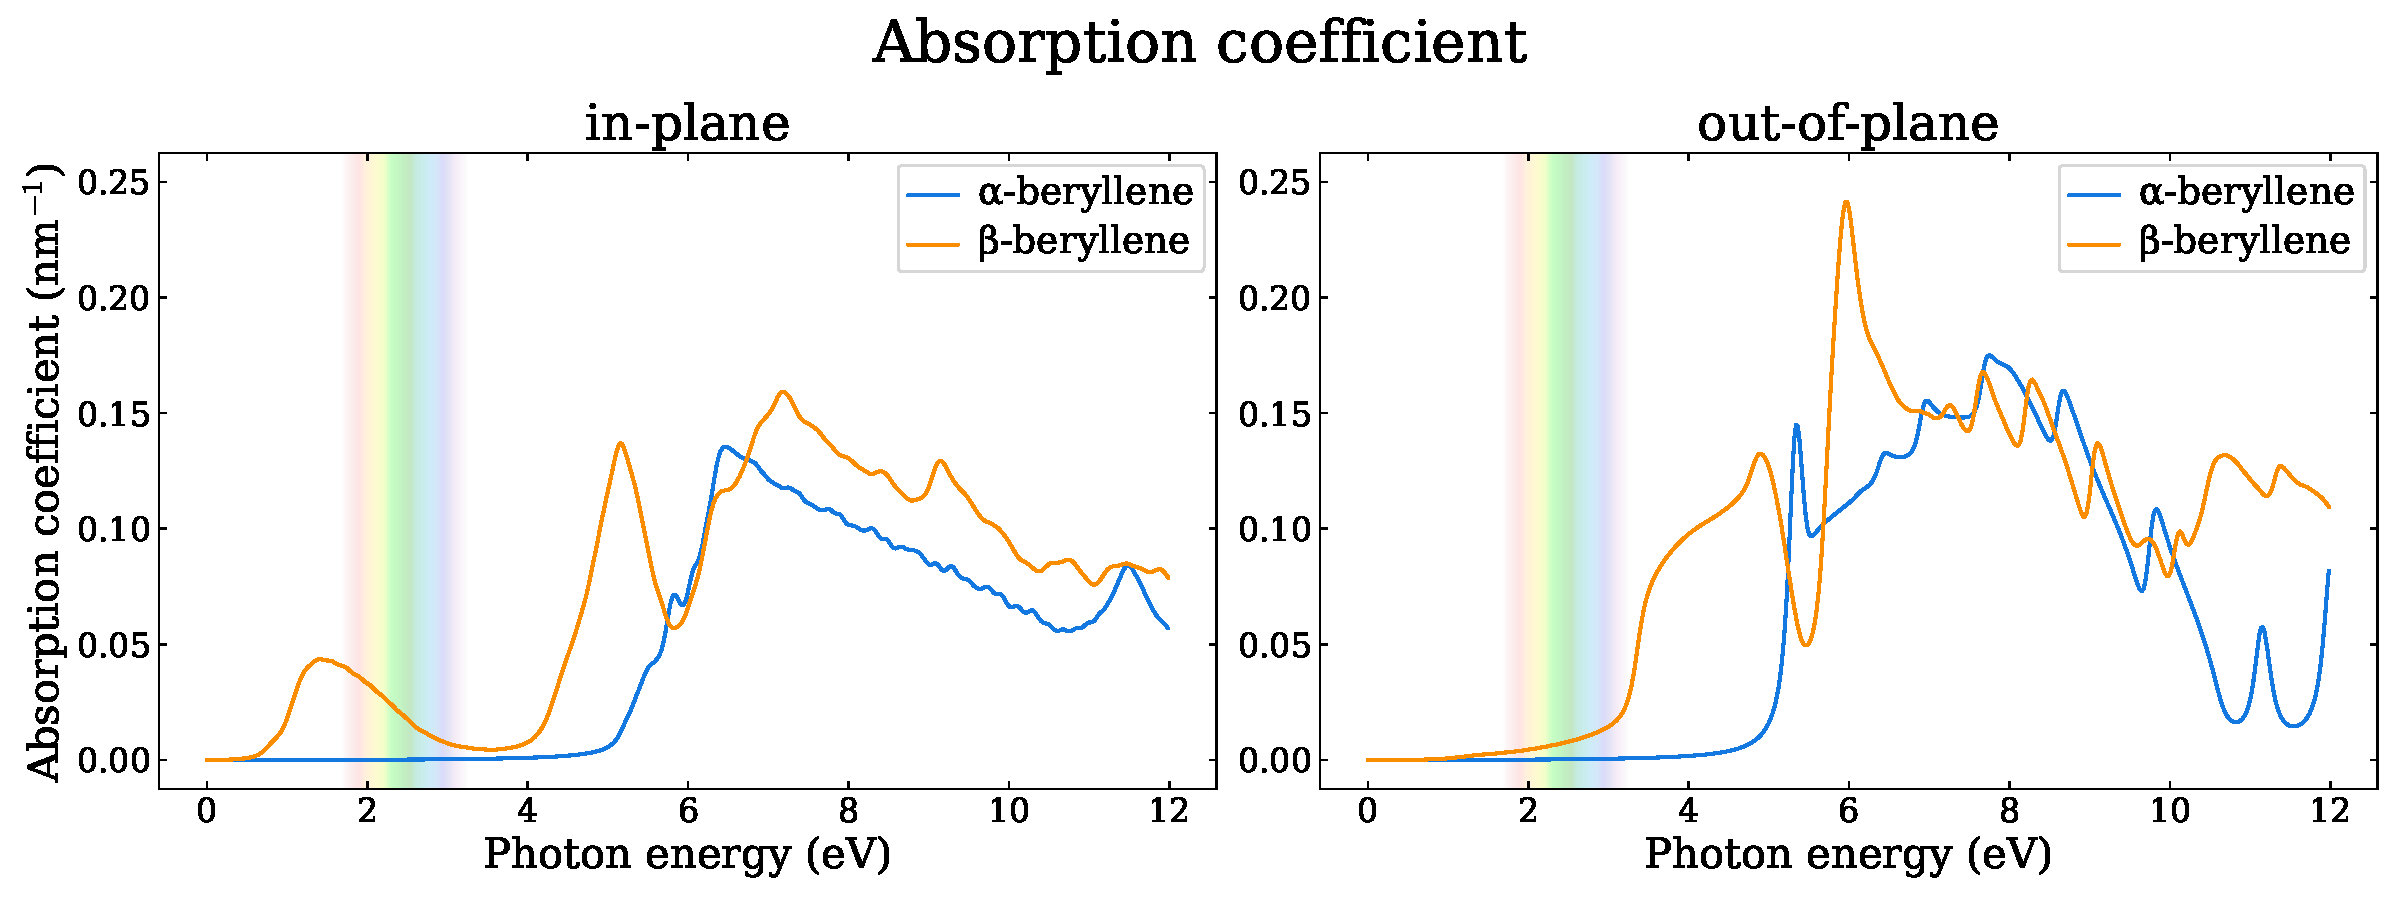
\includegraphics[width=0.95\textwidth]{figures_ch3/4.1_absorption.pdf}
\caption{The absorption coefficients for the in-plane and out-of-plane directions as functions of photon energy for $\alpha$-Beryllene and $\beta$-Beryllene.
The in-plane and out-of-plane curves correspond to the $xx$ and $zz$ components, respectively. The absorption coefficient is given in $\mathrm{nm}^{-1}$.
These spectra are from our calculations presented in chapter~\ref{cha:project_beryllene}.}
\label{absorption_coefficient_present_systems}
\end{figure}

The absorption coefficient spectra demonstrate differences between the two optical directions and between the two materials.
In the in-plane channel, $\beta$-Beryllene shows a stronger absorption response than $\alpha$-Beryllene over a broad photon-energy range,
whereas $\alpha$-Beryllene develops its main absorption only beyond the low-energy range and then forms a broader spectral feature.
In the out-of-plane channel, both materials develop stronger peak structures, while $\beta$-Beryllene still shows the stronger overall absorption.
These trends indicate that the optical attenuation depends on both the polarization direction and the crystal structure of the medium.

Once the electronic transitions generate different spectral weights along different directions,
the corresponding optical attenuation also acquires directional dependence~\cite{suk2024ultrafast}.

The low-energy increase of $\alpha_{\lambda}(\omega)$ identifies the beginning of the optical transitions.
As the photon energy increases, broader peaks emerge in the absorption spectrum.
These peaks indicate energy ranges where interband transitions contribute more strongly to the absorption process~\cite{elbanna20232d}.

Therefore, the absorption coefficient $\alpha_{\lambda}(\omega)$ reflects the directional excitation spectrum of the medium and characterizes the rate of optical attenuation~\cite{niu2024electronic,khan2025insight,zhang2024advanced,elbanna20232d}.
We next apply the same dielectric response to determine the refractive index $n_{\lambda}(\omega)$ and extinction coefficient $k_{\lambda}(\omega)$,
which describe the propagation of the attenuated wave.

\subsection{Refractive index and extinction coefficient}

The previous subsection described the absorption coefficient as the optical quantity that characterizes energy dissipation in the medium.
We now continue this description of light propagation in the medium by introducing the refractive index $n_{\lambda}(\omega)$ and the extinction coefficient $k_{\lambda}(\omega)$.
The refractive index determines the phase evolution,
whereas the extinction coefficient describes the attenuation of the wave amplitude.
Starting from the dielectric response,
we derive explicit expressions for $n_{\lambda}(\omega)$ and $k_{\lambda}(\omega)$~\cite{born2013principles,wooten2013optical,dressel2002electrodynamics,fox2010optical}.

For a monochromatic transverse mode polarized along the principal direction $\lambda$,
we first represent the electric field along the propagation coordinate $z$ as~\cite{politano2023spectroscopic}:

\begin{equation}
\begin{aligned}
    E_{\lambda}(z,t)
    &= E_{\lambda,0}\,
    \exp\left[\mathrm{i}\frac{\omega}{c}N_{\lambda}(\omega)z-\mathrm{i}\,\omega t\right]\\
    &= E_{\lambda,0}\,
    \exp\left[\mathrm{i}\frac{\omega}{c}n_{\lambda}(\omega)z\right]
    \exp\left[-\frac{\omega}{c}k_{\lambda}(\omega)z\right]
    \exp\left(-\mathrm{i}\,\omega t\right)
\end{aligned}
\label{monochromatic_wave_with_complex_refractive_index}
\end{equation}

here, $N_{\lambda}(\omega)$ denotes the complex refractive index.
Its real part $n_{\lambda}(\omega)$ denotes the refractive index,
and its imaginary part $k_{\lambda}(\omega)$ denotes the extinction coefficient.

This expression separates phase evolution from amplitude attenuation~\cite{wooten2013optical,dressel2002electrodynamics,born2013principles}.
In equation~\eqref{monochromatic_wave_with_complex_refractive_index},
the refractive index $n_{\lambda}(\omega)$ determines the phase evolution of the electromagnetic wave,
whereas the extinction coefficient $k_{\lambda}(\omega)$ describes the exponential attenuation of its amplitude in the medium.

For this mode and a scalar relative magnetic permeability $\mu_{\mathrm{r}}(\omega)$,
we write the relation between the complex refractive index and dielectric function as~\cite{born2013principles,wooten2013optical,dressel2002electrodynamics,politano2023spectroscopic}:

\begin{equation}
    N_{\lambda}^{2}(\omega)
    = \varepsilon_{\lambda\lambda}(\omega)\,\mu_{\mathrm{r}}(\omega)
\label{general_refractive_index_permeability_relation}
\end{equation}

here, $\mu_{\mathrm{r}}(\omega)$ is dimensionless.
Under the optical approximation $\mu_{\mathrm{r}}(\omega)\approx1$,
the relation reduces to~\cite{wooten2013optical,dressel2002electrodynamics,born2013principles}:

\begin{equation}
    N_{\lambda}^{2}(\omega)
    = \varepsilon_{\lambda\lambda}(\omega)
\label{nonmagnetic_refractive_index_dielectric_relation}
\end{equation}

We substitute equation~\eqref{direction_resolved_complex_dielectric_function}
and the definition of the complex refractive index $N_{\lambda}(\omega)$ in equation~\eqref{complex_refractive_index_for_absorption_coefficient}
into equation~\eqref{nonmagnetic_refractive_index_dielectric_relation},
and then separate the real and imaginary parts.
We therefore derive the coupled relations~\cite{wooten2013optical,dressel2002electrodynamics,fox2010optical}:

\begin{equation}
\begin{aligned}
    n_{\lambda}^{2}(\omega)-k_{\lambda}^{2}(\omega)
    &= \varepsilon_{1,\lambda\lambda}(\omega) \\
    2\,n_{\lambda}(\omega)\,k_{\lambda}(\omega)
    &= \varepsilon_{2,\lambda\lambda}(\omega)
\end{aligned}
\label{refractive_index_extinction_coefficient_auxiliary_relations}
\end{equation}

These two equations connect the refractive index $n_{\lambda}(\omega)$ and extinction coefficient $k_{\lambda}(\omega)$ to the real part $\varepsilon_{1,\lambda\lambda}(\omega)$ and imaginary part $\varepsilon_{2,\lambda\lambda}(\omega)$ of the dielectric function $\varepsilon_{\lambda\lambda}(\omega)$.

By solving these coupled relations,
we express the refractive index $n_{\lambda}(\omega)$ as~\cite{capper2019optical,cheng2025two,kim2024hyperspectral}:

\begin{equation}
    n_{\lambda}(\omega) = 
    \left[\frac{1}{2}\left(\sqrt{\varepsilon_{1,\lambda\lambda}^{2}(\omega)
        + \varepsilon_{2,\lambda\lambda}^{2}(\omega)}
        + \varepsilon_{1,\lambda\lambda}(\omega)\right)\right]^{1/2}
\label{refractive_index_from_dielectric_response}
\end{equation}

Similarly, we express the extinction coefficient $k_{\lambda}(\omega)$ as:

\begin{equation}
    k_{\lambda}(\omega) =
    \left[\frac{1}{2}\left(\sqrt{\varepsilon_{1,\lambda\lambda}^{2}(\omega)
        + \varepsilon_{2,\lambda\lambda}^{2}(\omega)}
        - \varepsilon_{1,\lambda\lambda}(\omega)\right)\right]^{1/2}
\label{extinction_coefficient_from_dielectric_response}
\end{equation}

With these expressions, we present the calculated refractive index $n_{\lambda}(\omega)$ spectra of $\alpha$-Beryllene and $\beta$-Beryllene:

\begin{figure}[htbp]
\centering
    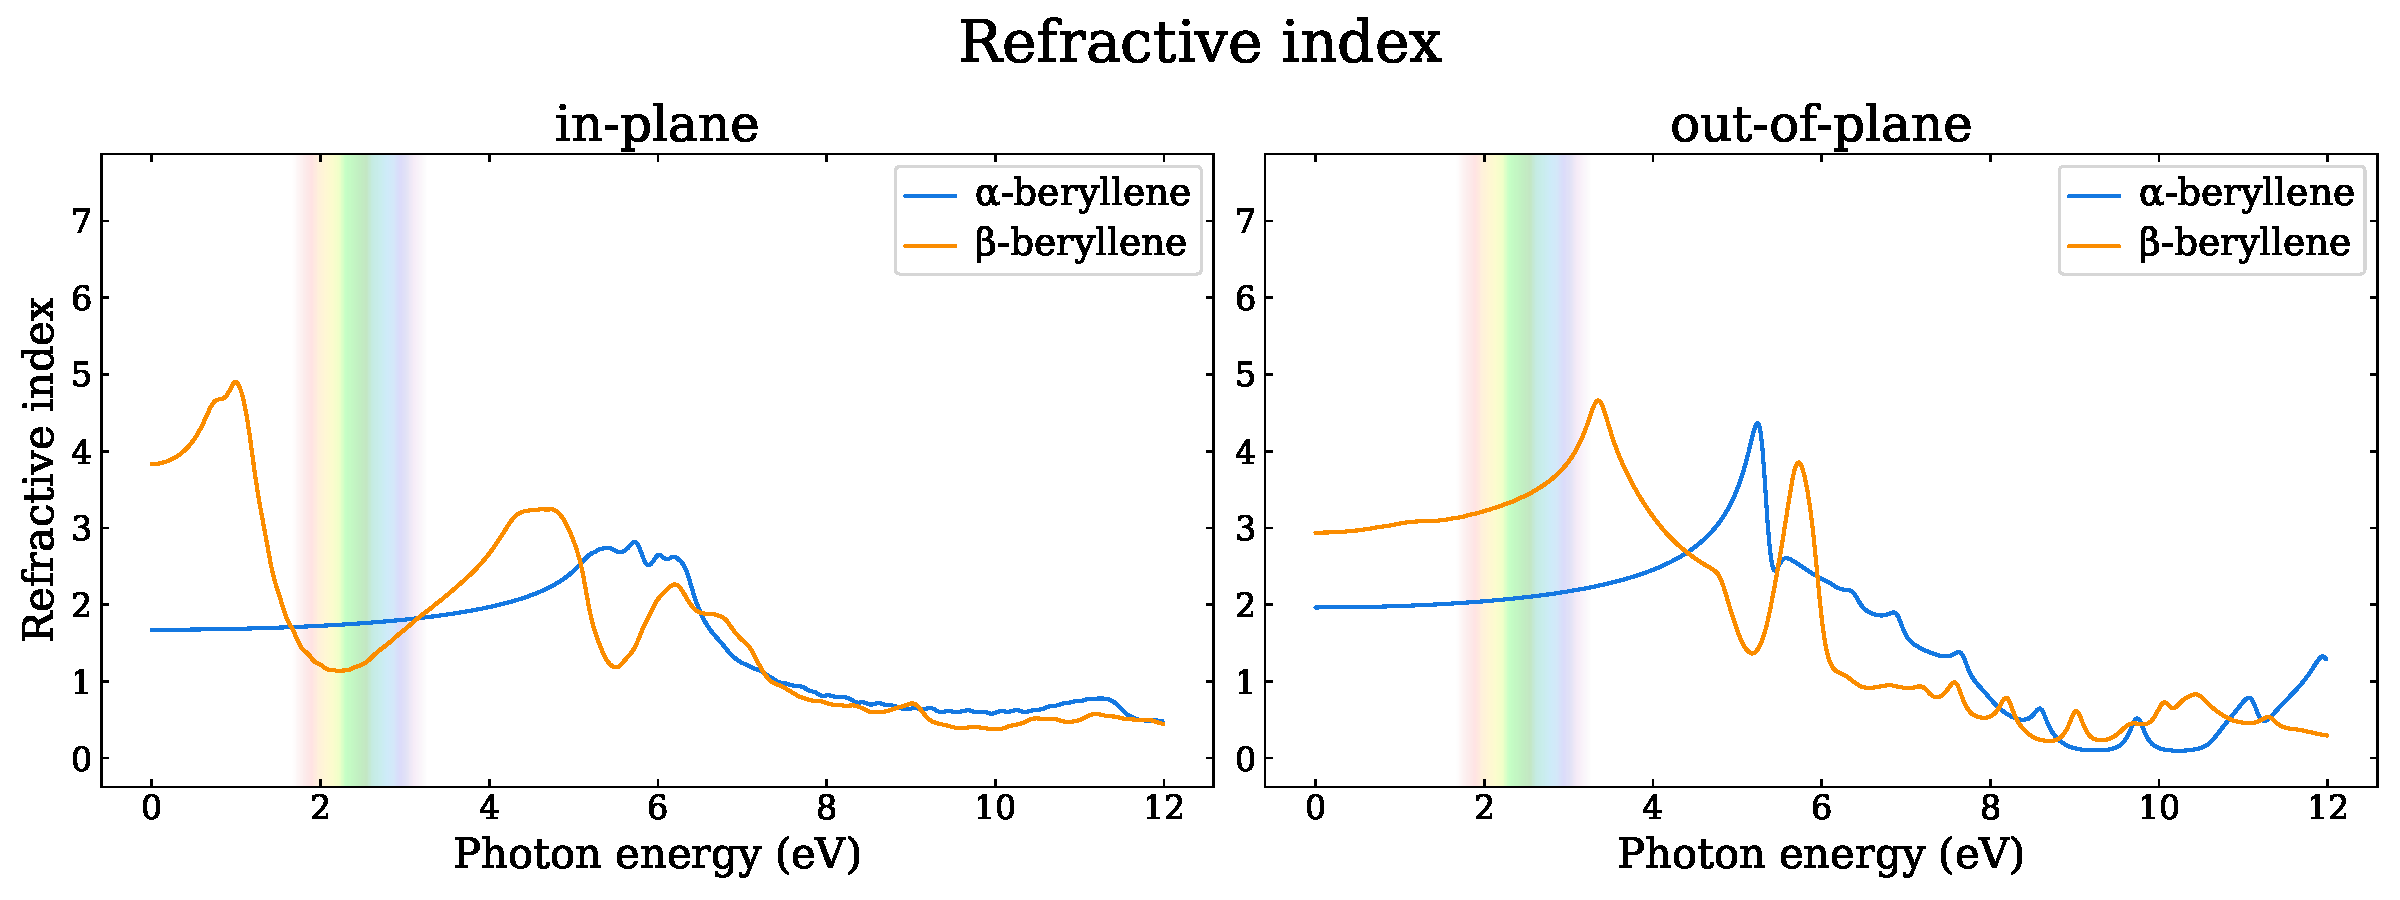
\includegraphics[width=0.95\textwidth]{figures_ch3/4.2_refractive.pdf}
\caption{The refractive indices for the in-plane and out-of-plane directions as functions of photon energy for $\alpha$-Beryllene and $\beta$-Beryllene.
The in-plane and out-of-plane curves correspond to the $xx$ and $zz$ components, respectively.
These spectra are from our calculations presented in chapter~\ref{cha:project_beryllene}.}
\label{refractive_index_present_systems}
\end{figure}

The refractive index spectra demonstrate distinct directional and structural contrasts.
In the in-plane channel, $\beta$-Beryllene develops two pronounced enhancements in the infrared and near-ultraviolet regions, with a minimum in the visible range, whereas $\alpha$-Beryllene varies more smoothly over the same interval.
In the out-of-plane channel, $\beta$-Beryllene remains stronger than $\alpha$-Beryllene over the infrared to near-ultraviolet range.
These trends indicate that the phase response depends on both the optical direction and the crystal structure of the medium.

We next present the extinction coefficient $k_{\lambda}(\omega)$ spectra,
which follow the absorptive part of the dielectric response more directly~\cite{wooten2013optical,dressel2002electrodynamics,fox2010optical}:

\begin{figure}[htbp]
\centering
    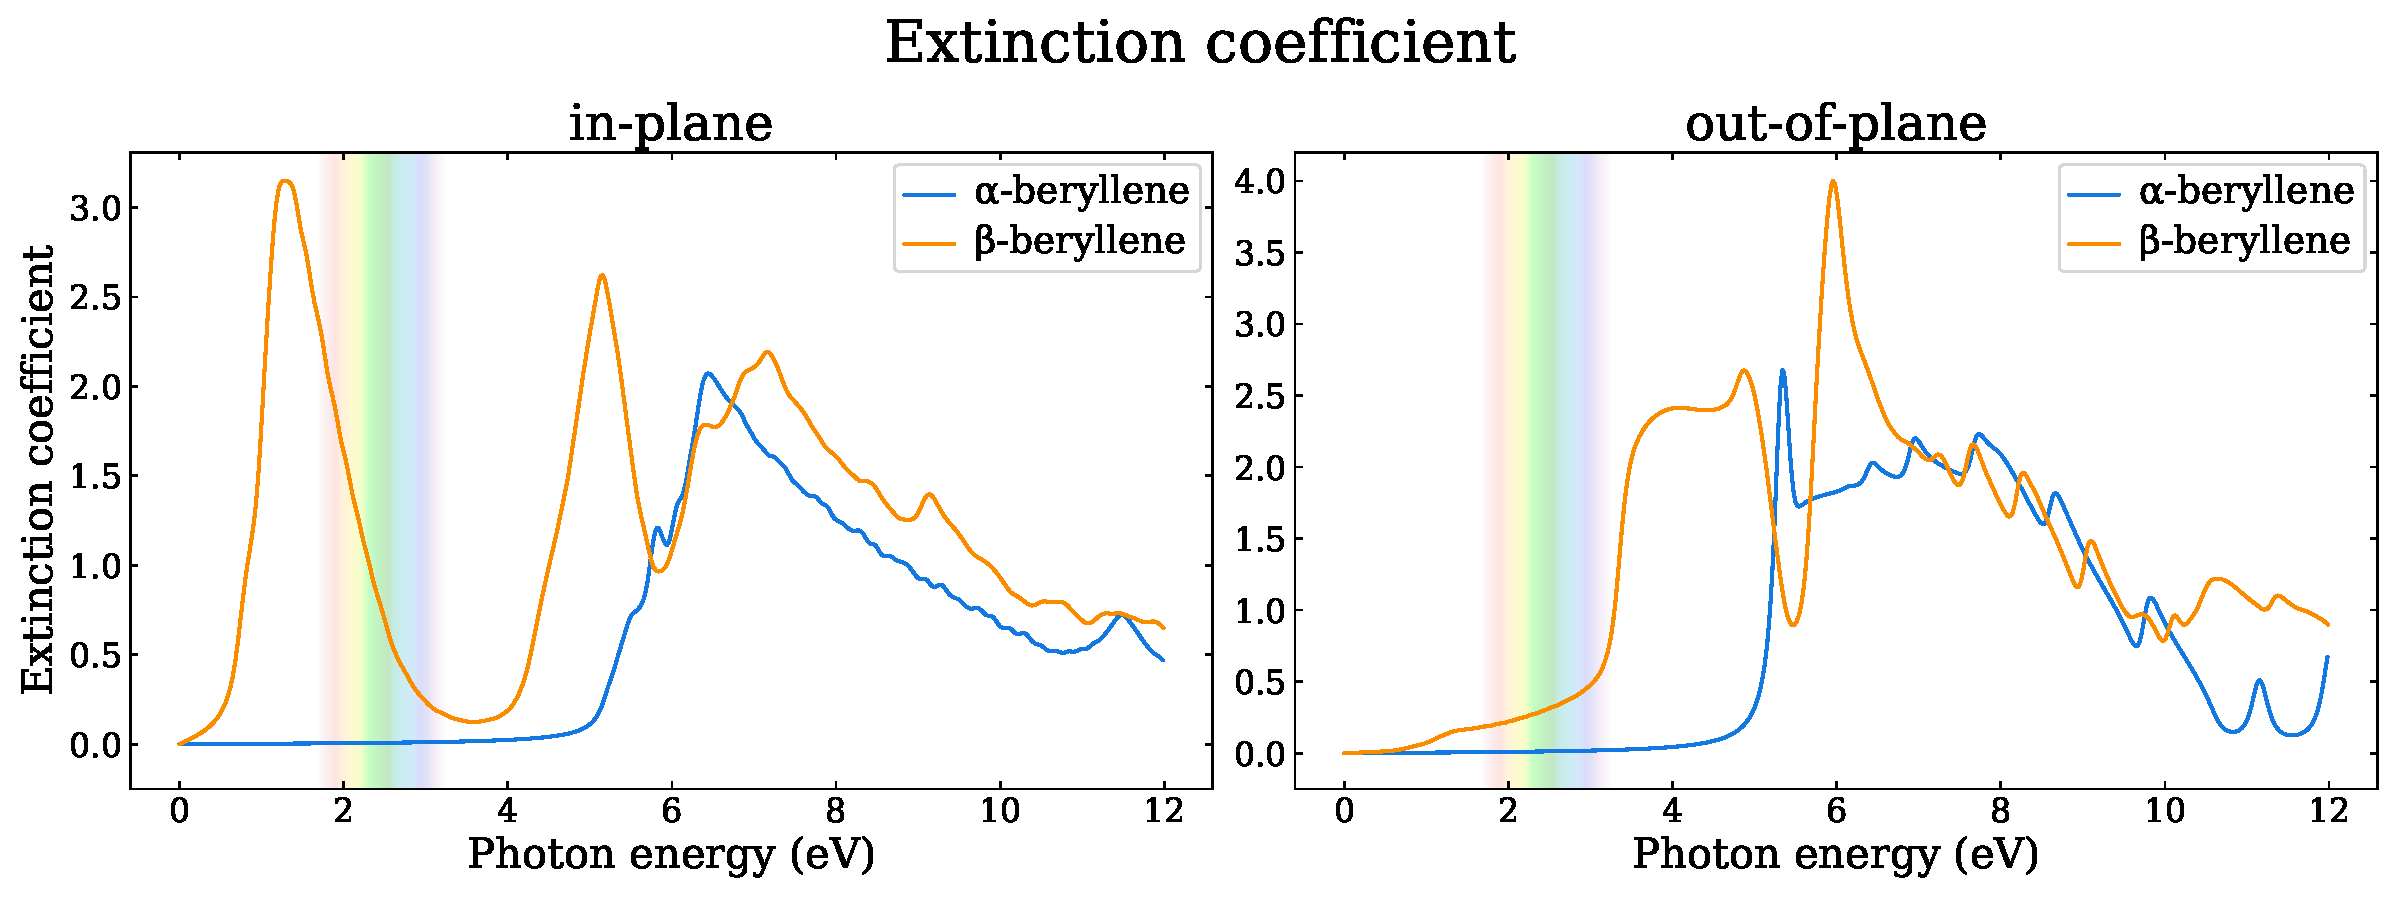
\includegraphics[width=0.95\textwidth]{figures_ch3/4.3_extinction.pdf}
\caption{The extinction coefficients for the in-plane and out-of-plane directions as functions of photon energy for $\alpha$-Beryllene and $\beta$-Beryllene.
The in-plane and out-of-plane curves correspond to the $xx$ and $zz$ components, respectively.
These spectra are from our calculations presented in chapter~\ref{cha:project_beryllene}.}
\label{extinction_coefficient_alpha_beta_beryllene}
\end{figure}

The extinction coefficient spectra demonstrate a similar directional contrast.
In the in-plane channel, $\beta$-Beryllene exhibits a strong infrared peak, followed by a pronounced trough from the visible to near-ultraviolet range and another strong feature in the ultraviolet region.
By contrast, $\alpha$-Beryllene remains weak at low photon energies and develops a broader ultraviolet response before gradually decreasing at higher energies.
In the out-of-plane channel, $\beta$-Beryllene is stronger than $\alpha$-Beryllene from the infrared to the near-ultraviolet range and reaches its largest response in the ultraviolet region.
Both phases then show oscillatory features and an overall decrease toward higher photon energies.
This behavior shows that amplitude attenuation also depends on both the optical direction and the crystal structure of the medium.

Accordingly, the refractive index $n_{\lambda}(\omega)$ and extinction coefficient $k_{\lambda}(\omega)$ connect the dielectric function to the interface response through the Fresnel equations~\cite{born2013principles,wooten2013optical,dressel2002electrodynamics}.
We next use them to determine the reflectivity, which transfers the bulk optical response to the interface.

\subsection{Reflectivity}

The previous subsection determined the refractive index $n_{\lambda}(\omega)$ and extinction coefficient $k_{\lambda}(\omega)$,
which characterize the phase propagation and amplitude attenuation in the medium.
We now turn from propagation inside the medium to reflection at its surface.

The reflectivity $R_{\lambda}(\omega)$ characterizes the fraction of incident electromagnetic energy reflected at the interface.
We then describe it through the Fresnel coefficient at normal incidence~\cite{born2013principles,wooten2013optical,dressel2002electrodynamics,fox2010optical}.

When an electromagnetic wave reaches the interface between two media,
the mismatch of optical response generates a reflected wave and a transmitted wave.
For a plane wave incident from an ambient medium with complex refractive index $N_{0,\lambda}(\omega)$ onto the present system with complex refractive index $N_{\lambda}(\omega)$,
the amplitude reflection coefficient at normal incidence takes the general form~\cite{born2013principles,wooten2013optical}:

\begin{equation}
    r_{\lambda}(\omega) =
    \frac{N_{\lambda}(\omega)-N_{0,\lambda}(\omega)}
    {N_{\lambda}(\omega)+N_{0,\lambda}(\omega)}
\label{normal_incidence_amplitude_reflection_coefficient_general}
\end{equation}

here, $r_{\lambda}(\omega)$ denotes the amplitude reflection coefficient,
$N_{0,\lambda}(\omega)$ denotes the complex refractive index of the incident medium,
and $N_{\lambda}(\omega)$ denotes the complex refractive index of the present medium.

For the optical quantities derived here,
we consider an interface between vacuum and a homogeneous semi-infinite effective medium with $\mu_{\mathrm{r}}(\omega)\approx1$.
The incident medium therefore satisfies $N_{0,\lambda}(\omega)=1$.
The resulting reflectivity is a parameter of this effective-medium model.
For a finite two-dimensional layer, the measured reflectance also depends on the thickness, substrate, and optical geometry.
At normal incidence on the structural plane, the electric field is in-plane.
The value obtained from $\varepsilon_{zz}(\omega)$ is therefore a formal out-of-plane response of the scalar model,
not a second normal-incidence channel of the layer.
With the complex refractive index $N_{\lambda}(\omega)$ in equation~\eqref{complex_refractive_index_for_absorption_coefficient},
we then write the amplitude reflection coefficient as:

\begin{equation}
    r_{\lambda}(\omega) =
    \frac{n_{\lambda}(\omega)-1+\mathrm{i}\,k_{\lambda}(\omega)}
    {n_{\lambda}(\omega)+1+\mathrm{i}\,k_{\lambda}(\omega)}
\label{normal_incidence_amplitude_reflection_coefficient_vacuum_interface}
\end{equation}

here, the refractive index $n_{\lambda}(\omega)$ determines the phase mismatch across the interface,
whereas the extinction coefficient $k_{\lambda}(\omega)$ represents the dissipative part of the optical response.
These two quantities together determine the reflected amplitude at the surface.

We next express the reflectivity $R_{\lambda}(\omega)$ as the reflected power ratio.
It equals the squared modulus of the amplitude reflection coefficient~\cite{born2013principles,wooten2013optical,dressel2002electrodynamics}:

\begin{equation}
    R_{\lambda}(\omega)
    = \left|r_{\lambda}(\omega)\right|^2
\label{reflectivity_from_amplitude_reflection_coefficient}
\end{equation}

After substituting equation~\eqref{normal_incidence_amplitude_reflection_coefficient_vacuum_interface},
this equation produces the reflectivity through the refractive index $n_\lambda(\omega)$ and the extinction coefficient $k_\lambda(\omega)$:

\begin{equation}
    R_{\lambda}(\omega) =
    \frac{\left[n_\lambda(\omega)-1\right]^2+k_\lambda^2(\omega)}
    {\left[n_\lambda(\omega)+1\right]^2+k_\lambda^2(\omega)}
\label{reflectivity_from_refractive_index_and_extinction_coefficient}
\end{equation}

This equation links the surface reflection to the refractive index $n_{\lambda}(\omega)$ and the extinction coefficient $k_{\lambda}(\omega)$.
A larger mismatch between $n_{\lambda}(\omega)$ and the vacuum value enhances reflection,
whereas $k_{\lambda}(\omega)$ modifies the reflected intensity through optical dissipation.
Therefore, the reflectivity $R_{\lambda}(\omega)$ characterizes the reflected optical response at a specific photon energy.

The following figure presents the calculated reflectivity $R_{\lambda}(\omega)$ spectra of $\alpha$-Beryllene and $\beta$-Beryllene for the in-plane and out-of-plane directions:

\begin{figure}[htbp]
\centering
    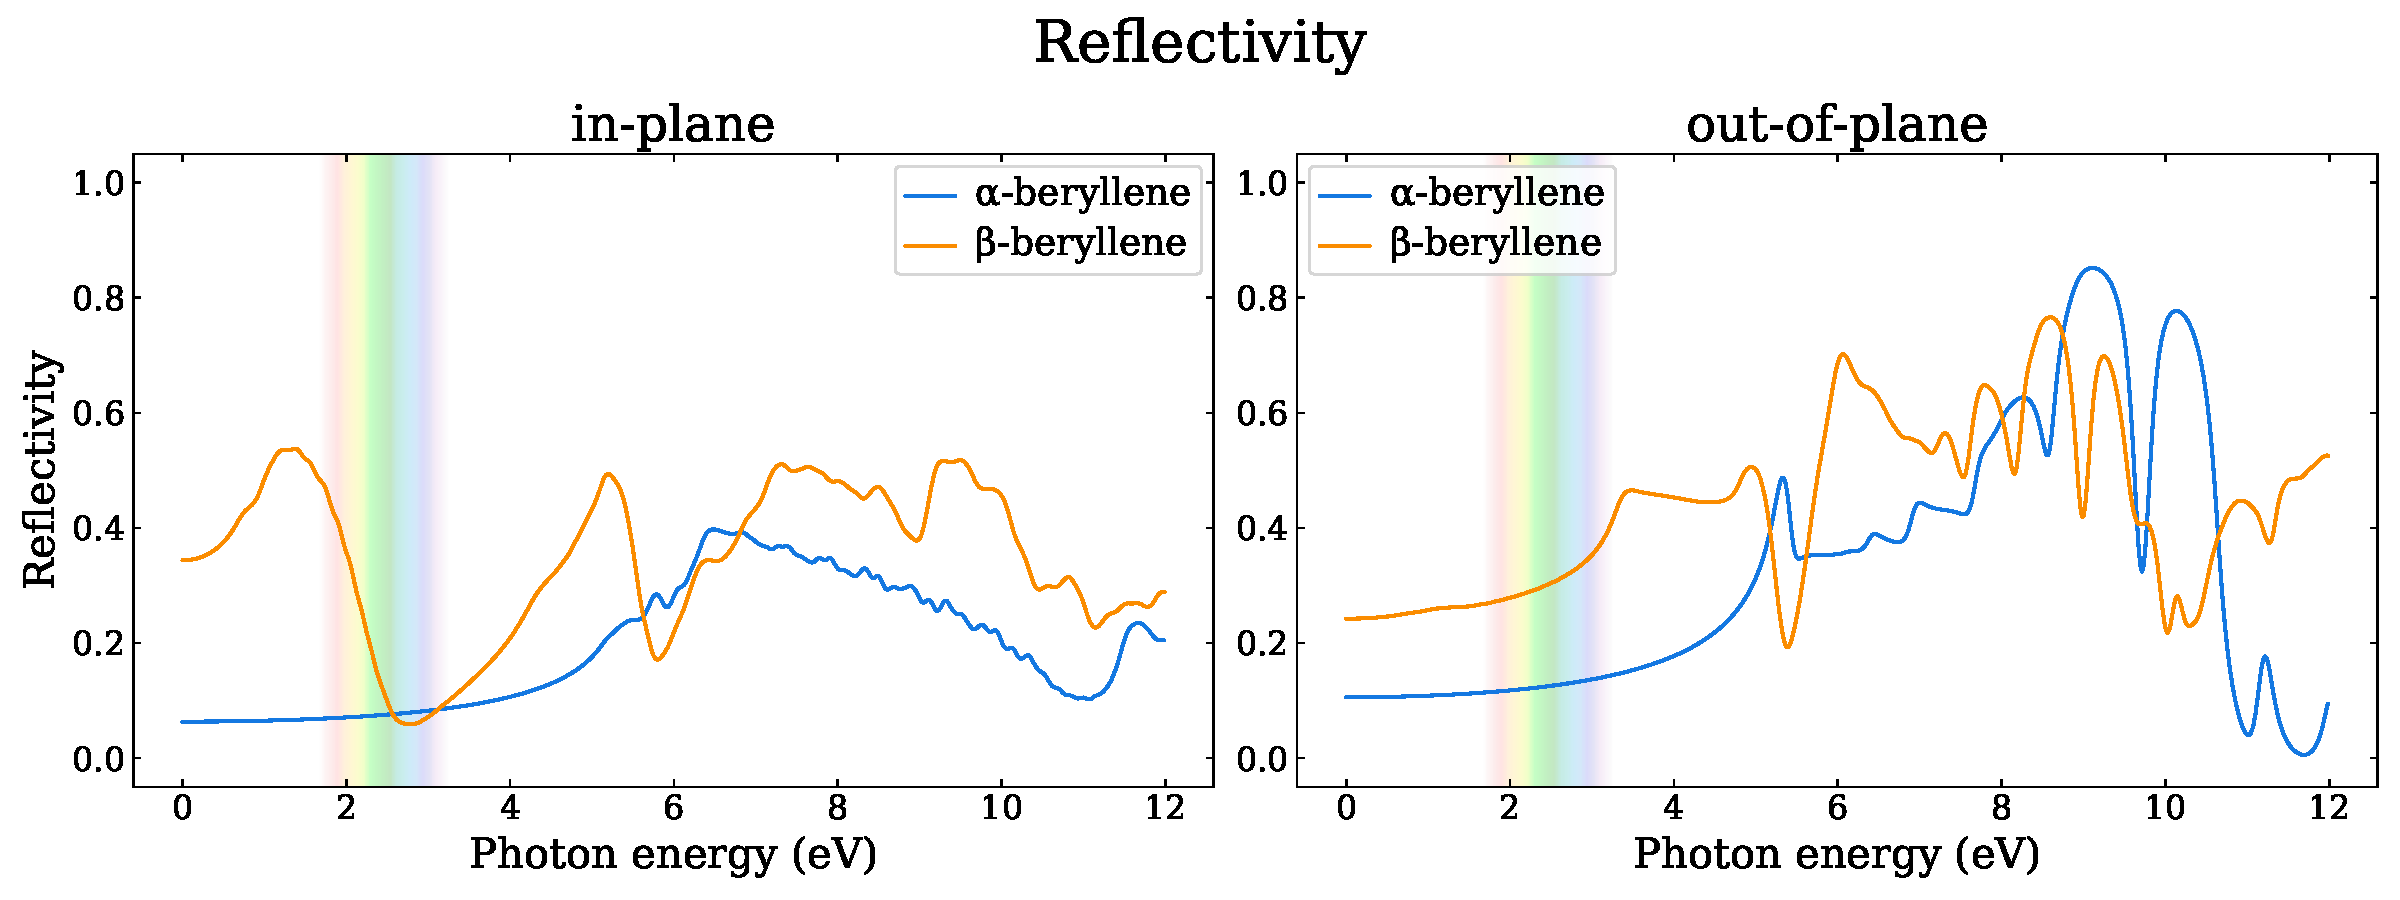
\includegraphics[width=0.95\textwidth]{figures_ch3/4.4_reflectivity.pdf}
\caption{The reflectivities for the in-plane and out-of-plane directions as functions of photon energy for $\alpha$-Beryllene and $\beta$-Beryllene.
The in-plane and out-of-plane curves correspond to the $xx$ and $zz$ components, respectively. The reflectivities are evaluated within the effective-medium model described in the text.
These spectra are from our calculations presented in chapter~\ref{cha:project_beryllene}.}
\label{reflectivity_alpha_beta_beryllene}
\end{figure}

The reflectivity spectra follow the directional contrast already demonstrated in the extinction coefficient.
In the in-plane channel, $\beta$-Beryllene exhibits strong low-energy reflection, followed by a pronounced minimum across the visible range and renewed strong reflection from the near-ultraviolet into the ultraviolet region,
whereas $\alpha$-Beryllene varies more smoothly with a broad intermediate-energy feature.
In the out-of-plane channel, $\beta$-Beryllene remains stronger over the low-energy range and then develops a series of rapid oscillations toward higher photon energies,
while $\alpha$-Beryllene shows pronounced peaks in the ultraviolet region.
These trends reflect the combined role of the refractive index $n_{\lambda}(\omega)$ and the extinction coefficient $k_{\lambda}(\omega)$ in determining the surface reflectivity.

We next turn to the energy-loss spectrum $L_{\lambda}(\omega)$ and examine the longitudinal loss response of the medium.

\subsection{Energy-loss spectrum}

The previous subsection introduced the reflectivity $R_{\lambda}(\omega)$ as the optical response of the surface,
characterized by the refractive index $n_{\lambda}(\omega)$ and the extinction coefficient $k_{\lambda}(\omega)$.
We now move from surface reflection to energy dissipation inside the medium by examining the energy-loss spectrum $L_{\lambda}(\omega)$.

The energy-loss spectrum $L_{\lambda}(\omega)$ characterizes the energy transferred from an external probe to the medium at an energy transfer $\hbar\omega$.
Here, we consider a longitudinal perturbation along the principal direction $\lambda$ in the local, long-wavelength limit.
This loss function describes the corresponding bulk response relevant to electron energy-loss spectroscopy;
finite momentum and surface contributions require the appropriate scattering geometry.

We first express this principal-axis loss function as~\cite{dressel2002electrodynamics,wooten2013optical,fox2010optical,onida2002electronic}:

\begin{equation}
    L_{\lambda}(\omega)=
    \mathrm{Im}\left[-\frac{1}{\varepsilon_{\lambda\lambda}(\omega)}\right]
\label{energy_loss_spectrum_from_inverse_dielectric_function}
\end{equation}

This expression indicates that the energy-loss spectrum $L_{\lambda}(\omega)$ is governed by the inverse dielectric function $1/\varepsilon_{\lambda\lambda}(\omega)$.
For a medium, it therefore follows not only the imaginary part $\varepsilon_{2,\lambda\lambda}(\omega)$,
but also the screening effect determined by the full complex dielectric function $\varepsilon_{\lambda\lambda}(\omega)$.

For a weakly damped longitudinal collective excitation,
a loss peak can occur near a zero of $\varepsilon_{1,\lambda\lambda}(\omega)$ when $\varepsilon_{2,\lambda\lambda}(\omega)$ is small.
Interband excitations also contribute to the loss spectrum,
so a peak alone does not establish a plasmon~\cite{dressel2002electrodynamics,onida2002electronic}.

Substituting equation~\eqref{direction_resolved_complex_dielectric_function} into equation~\eqref{energy_loss_spectrum_from_inverse_dielectric_function}, we then obtain the explicit expression adopted in the present work:

\begin{equation}
    L_{\lambda}(\omega) =
    \frac{\varepsilon_{2,\lambda\lambda}(\omega)}
    {\varepsilon_{1,\lambda\lambda}^{2}(\omega)
    + \varepsilon_{2,\lambda\lambda}^{2}(\omega)}
\label{energy_loss_spectrum_from_dielectric_function}
\end{equation}

This expression separates the dissipative channel from the dielectric screening.
The imaginary part $\varepsilon_{2,\lambda\lambda}(\omega)$ enters both the numerator and the denominator.
At $\varepsilon_{1,\lambda\lambda}(\omega)=0$ and finite positive $\varepsilon_{2,\lambda\lambda}(\omega)$,
the loss function is $L_{\lambda}(\omega)=1/\varepsilon_{2,\lambda\lambda}(\omega)$.
Therefore, a large imaginary part does not by itself produce a strong loss peak.
The loss spectrum describes longitudinal screening and complements the transverse absorption and reflection responses~\cite{dressel2002electrodynamics,onida2002electronic}.

The following figure presents the calculated energy-loss $L_{\lambda}(\omega)$ spectra of $\alpha$-Beryllene and $\beta$-Beryllene for the in-plane and out-of-plane directions:

\begin{figure}[htbp]
\centering
    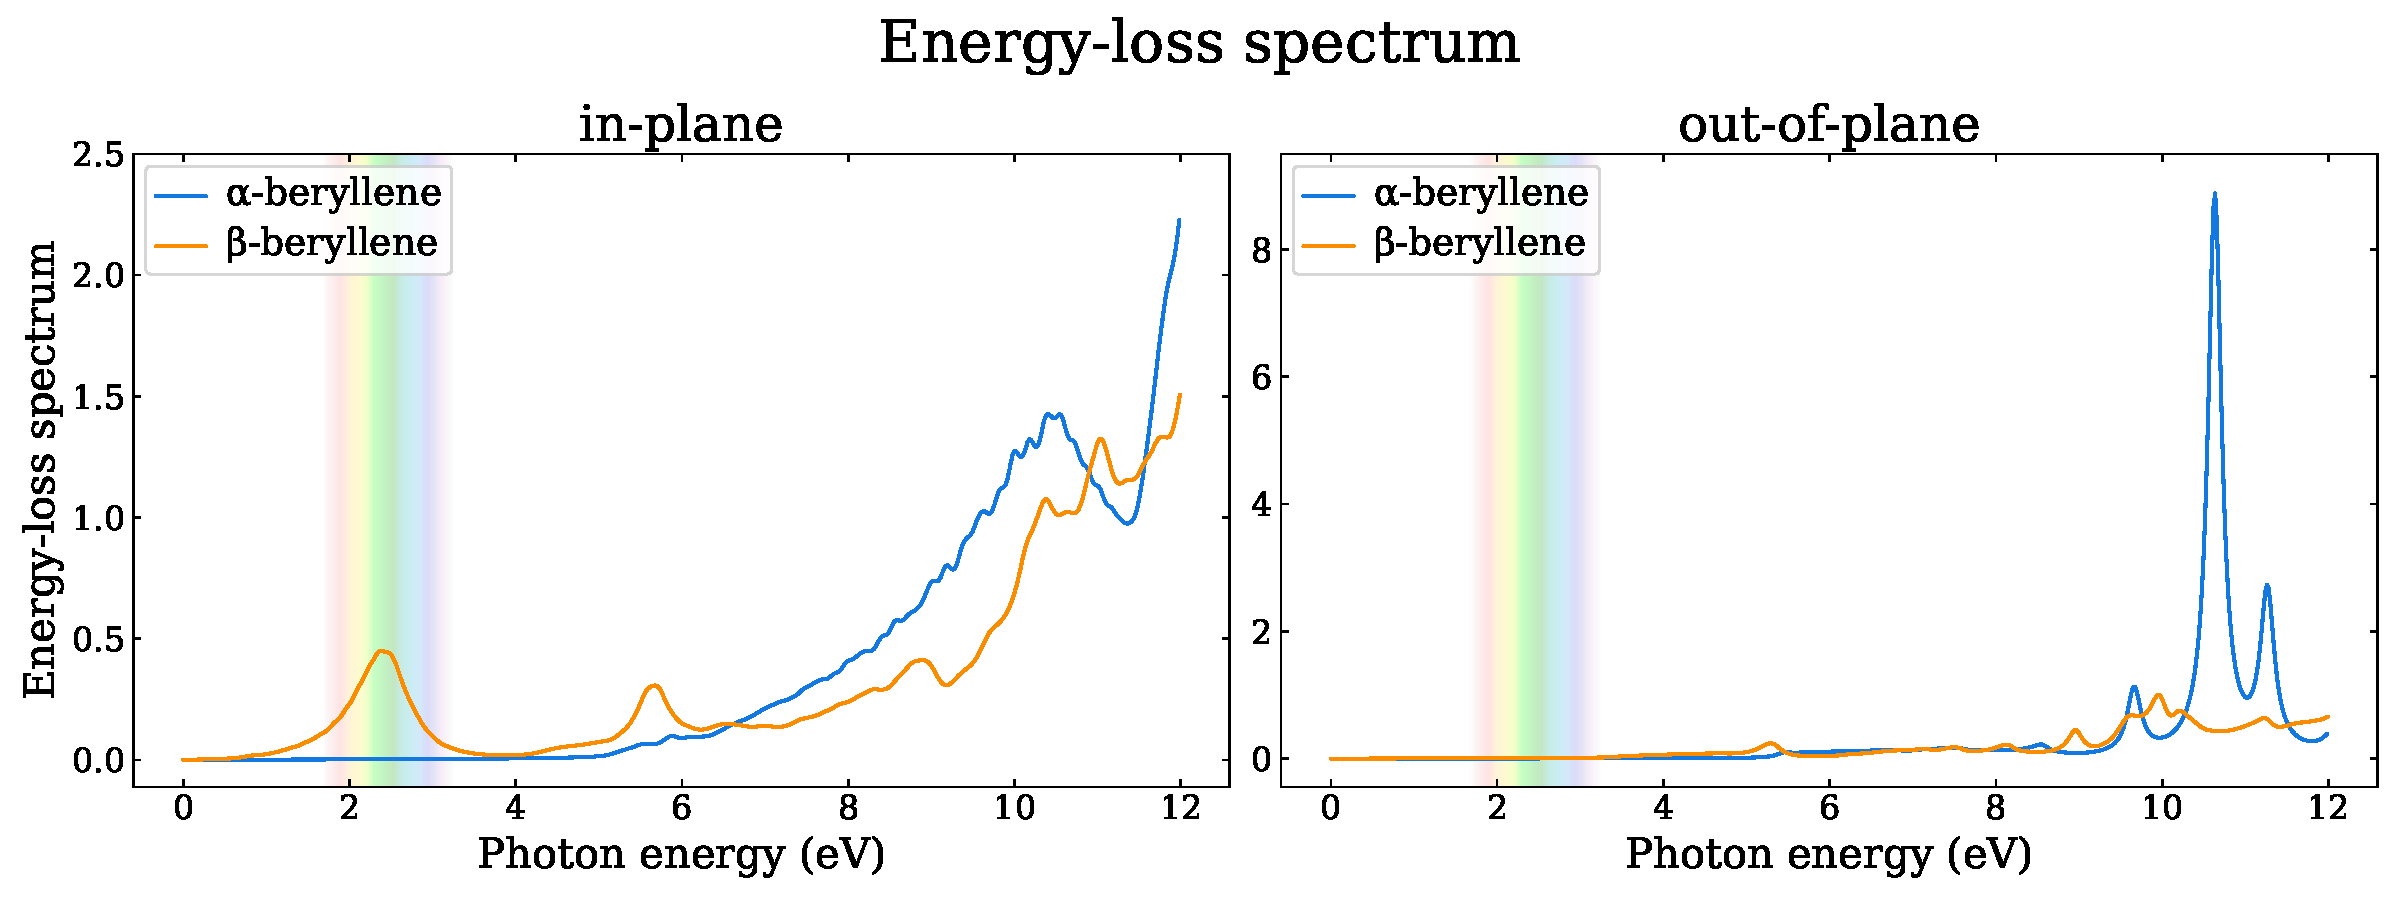
\includegraphics[width=0.95\textwidth]{figures_ch3/4.5_energy-loss.pdf}
\caption{The energy-loss spectra for the in-plane and out-of-plane directions as functions of photon energy for $\alpha$-Beryllene and $\beta$-Beryllene.
The in-plane and out-of-plane curves correspond to the $xx$ and $zz$ components, respectively.
These spectra are from our calculations presented in chapter~\ref{cha:project_beryllene}.}
\label{energy_loss_spectrum_alpha_beta_beryllene}
\end{figure}

The energy-loss spectra demonstrate clear directional and structural contrasts.
In the in-plane channel, $\beta$-Beryllene develops a visible-range peak and a stronger response in the deep-ultraviolet region,
whereas $\alpha$-Beryllene remains weak at low photon energy and rises toward the upper end of the plotted range.
In the out-of-plane channel, both materials remain weak in the visible range and develop stronger loss features at higher energies.
The deep-ultraviolet peak of $\alpha$-Beryllene is stronger than that of $\beta$-Beryllene.

These results demonstrate that the energy-loss spectrum $L_{\lambda}(\omega)$ varies with both the response direction and the crystal structure of the medium.
As $L_{\lambda}(\omega)$ follows the inverse dielectric function,
its peaks identify energy ranges with a strong longitudinal loss response.

Consequently, we arrive at the final optical quantity derived from the dielectric function $\varepsilon_{\lambda\lambda}(\omega)$ and complete the chain from the absorption coefficient $\alpha_{\lambda}(\omega)$,
to the refractive index $n_{\lambda}(\omega)$ and extinction coefficient $k_{\lambda}(\omega)$, to the reflectivity $R_{\lambda}(\omega)$, and finally to the energy-loss spectrum $L_{\lambda}(\omega)$.
